%% LyX 2.0.4 created this file.  For more info, see http://www.lyx.org/.
%% Do not edit unless you really know what you are doing.
\documentclass[11pt,oneside,english]{amsart}
\usepackage[T1]{fontenc}
\usepackage[latin9]{inputenc}
\usepackage{geometry}
\geometry{verbose, margin = 1in}
\usepackage{amsthm}
\usepackage{tikz}
\usepackage{array}
\usetikzlibrary{arrows}
\usepackage{amsfonts}
\usepackage{caption}
\usepackage{subcaption}
\usepackage{multicol}

\setlength{\parskip}{0.5pc}


\makeatletter
%%%%%%%%%%%%%%%%%%%%%%%%%%%%%% Textclass specific LaTeX commands.
\numberwithin{equation}{section}
\numberwithin{figure}{section}
\theoremstyle{plain}
\newtheorem{thm}{\protect\theoremname}
  \theoremstyle{definition}
  \newtheorem{defn}[thm]{\protect\definitionname}
  \theoremstyle{plain}
  \newtheorem{lem}[thm]{\protect\lemmaname}
  \setlength\parindent{0pt}
  \newtheorem{assumpt}{\protect \assumptionname}
  \theoremstyle{plain}
  \newtheorem{inv}{\protect \invariantname}

\makeatother

\usepackage{babel}
  \providecommand{\definitionname}{Definition}
  \providecommand{\lemmaname}{Lemma}
  \providecommand{\theoremname}{Theorem}
  \providecommand{\assumptionname}{Assumption}
  \providecommand{\invariantname}{Invariant}

\definecolor{lightgray}{RGB}{240, 240, 240}
\definecolor{mediumgray}{RGB}{220, 220, 220}

\begin{document}

\title{Treasure Hunting}
\author{Casey O'Brien (cmobrien@mit.edu)}


\maketitle

Our goal is to solve the collaborative search on the plane problem. In this problem, there are $k$ identical agents, initially located at the origin, and a treasure located Manhattan distance $D$ from the origin. Their goal is to locate the treasure as efficiently as possible, both in terms of $D$ and $k$. 

The agents all move synchronously. In a single time step, an agent can take one step to the north, east, south, or west, or stay in the same location. Our goal is to develop an algorithm for the agents to locate the treasure in the optimal time, $O(D + D^2/k)$, when the agents have only weak capabilities. Specifically, our agents will only have constant memory, and very limited communcation abilities. The only communication allowed will be \textit{loneliness detection}, which means that when an agent is in a cell, it knows whether or not it is alone. Additionally, the agents will be able to sense whether their current cell is the origin.

\section{Introduction}

We will describe the algorithm \textsc{Rectangle-Search}. It consists of three phases. The first phase is the \textit{Separation Phase}. This is the only probabilistic phase. In this phase, the agents work to become alone in a cell, so that they can then make use of their loneliness detection ability.

The second phase is the \textit{Allocation Phase}. In this phase, the agents divide up into teams of five, and each agent is assigned a role within its team. The final phase is the \textit{Search Phase}. In this phase, the agents actually begin to search the plane for the treasure by collectively searching from the origin outwards.

Since the \textit{Search Phase} comprises the majority of the algorithm, we will describe it first, in Section 2. In Section 3, we will describe the \textit{Separation Phase}, and in Section 4 we will describe the \textit{Allocation Phase}.

\section{Search Phase}

Since the \textit{Separation} and \textit{Allocation Phases} actually happen before the \textit{Search} phase in \textit{Rectangle-Search}, we will need to make some assumptions about the behavior of the agents entering the \textit{Search Phase} before we can proceed to describe this phase. In later sections, we will see how the early phases actually allow these assumptions to be valid.

\subsection{Assumptions} We make the following assumptions.

\begin{assumpt} The agents are broken into teams of five, and each agent knows its role within its team.
\end{assumpt}

\begin{assumpt} Each agent knows whether or not it belongs to the first team.
\end{assumpt}

\begin{assumpt} All the agents begin at the origin. A search team can leave the origin on any even time step at least twelve steps after the previous team left. The second search team must leave the origin before the first search team completes exploring level 2.
\end{assumpt}

\subsection{Exploring Levels}

Define \textit{level $d$} to be the set of all cells which are exactly $d$ steps from the origin. The general idea behind the algorithm is that search teams will concurrently search different levels, starting from level $1$ and making their way outwards. Once a team finishes searching a level, it will move outwards again and explored the next unexplored level.

In order for this algorithm to work, the agents will have coordinate with each other very carefully. To do this, each agent of a search team is assigned one of five roles: the explorer, or the north, east, south, or west guide.

\begin{figure}
\begin{tabular}{c c}
\begin{subfigure}[b]{.5\textwidth}
\centering
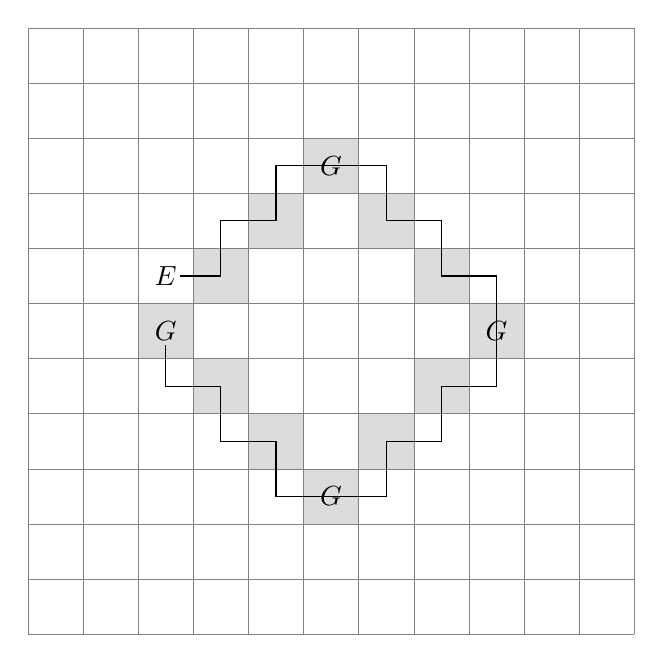
\begin{tikzpicture}[scale=0.7]

\fill[mediumgray] (5,2) rectangle (6,3);
\fill[mediumgray] (4,3) rectangle (5,4);
\fill[mediumgray] (6,3) rectangle (7,4);
\fill[mediumgray] (3,4) rectangle (4,5);
\fill[mediumgray] (7,4) rectangle (8,5);
\fill[mediumgray] (2,5) rectangle (3,6);
\fill[mediumgray] (8,5) rectangle (9,6);
\fill[mediumgray] (5,8) rectangle (6,9);
\fill[mediumgray] (4,7) rectangle (5,8);
\fill[mediumgray] (6,7) rectangle (7,8);
\fill[mediumgray] (3,6) rectangle (4,7);
\fill[mediumgray] (7,6) rectangle (8,7);

\draw [help lines] (0,0) grid (11, 11);
\node(g1) at (2.5, 5.5){$G$};
\node(g2) at (5.5, 8.5){$G$};
\node(g3) at (5.5, 2.5){$G$};
\node(g4) at (8.5, 5.5){$G$};
\node(e) at (2.5, 6.5){$E$};
\draw  (2.75, 6.5)
    -- (3.5, 6.5)
    -- (3.5, 7.5)
    -- (4.5, 7.5)
    -- (4.5, 8.5)
    -- (5.5, 8.5)
    % At north guide
    -- (6.5, 8.5)
    -- (6.5, 7.5)
    -- (7.5, 7.5)
    -- (7.5, 6.5)
    -- (8.5, 6.5)
    -- (8.5, 5.5)
    % At east guide
    -- (8.5, 4.5)
    -- (7.5, 4.5)
    -- (7.5, 3.5)
    -- (6.5, 3.5)
    -- (6.5, 2.5)
    -- (5.5, 2.5)
    % At south guide
    -- (4.5, 2.5)
    -- (4.5, 3.5)
    -- (3.5, 3.5)
    -- (3.5, 4.5)
    -- (2.5, 4.5)
    -- (2.5, 5.25);
\end{tikzpicture}
\caption{}
\end{subfigure}
&
\begin{subfigure}[b]{0.5\textwidth}
\centering
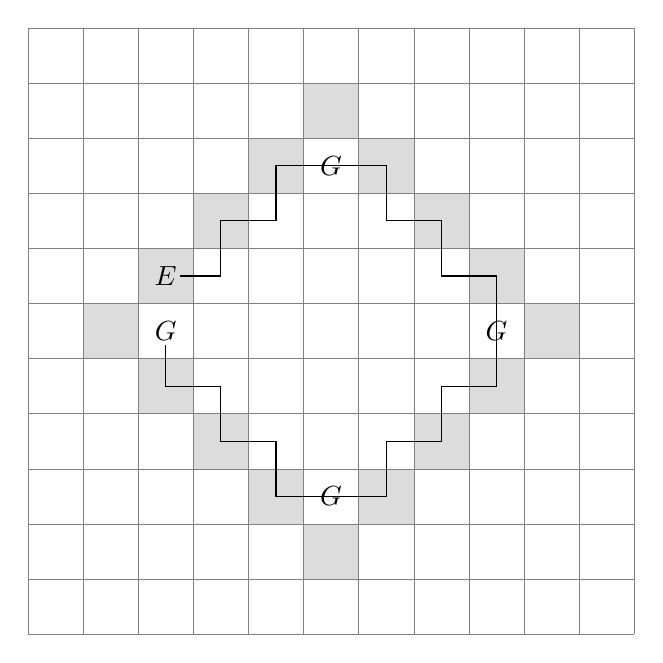
\begin{tikzpicture}[scale=0.7]

\fill[mediumgray] (5,1) rectangle (6,2);
\fill[mediumgray] (4,2) rectangle (5,3);
\fill[mediumgray] (6,2) rectangle (7,3);
\fill[mediumgray] (3,3) rectangle (4,4);
\fill[mediumgray] (7,3) rectangle (8,4);
\fill[mediumgray] (2,4) rectangle (3,5);
\fill[mediumgray] (8,4) rectangle (9,5);
\fill[mediumgray] (1,5) rectangle (2,6);
\fill[mediumgray] (9,5) rectangle (10,6);
\fill[mediumgray] (5,9) rectangle (6,10);
\fill[mediumgray] (4,8) rectangle (5,9);
\fill[mediumgray] (6,8) rectangle (7,9);
\fill[mediumgray] (3,7) rectangle (4,8);
\fill[mediumgray] (7,7) rectangle (8,8);
\fill[mediumgray] (2,6) rectangle (3,7);
\fill[mediumgray] (8,6) rectangle (9,7);
\draw [help lines] (0,0) grid (11, 11);
\node(g1) at (2.5, 5.5){$G$};
\node(g2) at (5.5, 8.5){$G$};
\node(g3) at (5.5, 2.5){$G$};
\node(g4) at (8.5, 5.5){$G$};
\node(e) at (2.5, 6.5){$E$};
\draw  (2.75, 6.5)
    -- (3.5, 6.5)
    -- (3.5, 7.5)
    -- (4.5, 7.5)
    -- (4.5, 8.5)
    -- (5.5, 8.5)
    % At north guide
    -- (6.5, 8.5)
    -- (6.5, 7.5)
    -- (7.5, 7.5)
    -- (7.5, 6.5)
    -- (8.5, 6.5)
    -- (8.5, 5.5)
    % At east guide
    -- (8.5, 4.5)
    -- (7.5, 4.5)
    -- (7.5, 3.5)
    -- (6.5, 3.5)
    -- (6.5, 2.5)
    -- (5.5, 2.5)
    % At south guide
    -- (4.5, 2.5)
    -- (4.5, 3.5)
    -- (3.5, 3.5)
    -- (3.5, 4.5)
    -- (2.5, 4.5)
    -- (2.5, 5.25);
\end{tikzpicture}
\caption{}
\end{subfigure}
\end{tabular}
\caption{TEST}
\end{figure}

Say that a search team is going to explore level $d$. The guides will position themselves on their corresponding axis exactly $d$ steps from the origin, and the explorer positions himself one cell above the west guide. Now, in order to explore level $d$, the explorer begins by alternating taking steps to the east and north, until it reaches the north guide, at which point it begins alternating taking steps to the east and south until it reaches the east guide, and so on. After $8d - 1$ steps, the agent will have reached the west guide, and all cells at level $d$ will have been explored. Figure 1.1(a) shows an example of the path of the explorer for $d = 3$, where the cells at level 3 are highlighted.

In fact, we note that all cells at level $d + 1$ will have also been explored, except for those lying exactly one step further from the origin than the guides. To demonstrate this point, Figure 1.1(b) shows the path of an explorer who is exploring level 3, with the level 4 cells highlighted. Soon we will see that these cells along the axes will be explored by the guides, and so it is unnecessary to have any team explore level $d + 1$. As a result, we only need to designate a search team to explore every other level.

\subsection{Progression}

Now we need to make sure that the guides use only constant memory. As described above, the guides need to move $d$ steps from the origin before the search at level $d$ can begin. In order to do this using only a constant amount of memory, the guides will make use of guides from other search teams.

The \textit{Search Phase} begins with the first team exploring level 2. Their search begins with the explorer walking out along the west axis, directly followed by the west guide. The other guides walk in sync with the west guide, along their respective axes. Once the explorer reaches the point two steps to the left of the origin, it takes a step upwards. After this step, the team is in position to begin exploration of level $2$, and the explorer proceeds to search the level as described above.

While the first team is exploring level 2, the second team begins to execute the \textit{Search Phase}. As before, the explorer leads the west guide out along the west axis, and all other guides walk out in sync with the west guide. These agents are not actually aware that they are the second team (they only know that they are not the first team), so we need a strategy to let the agents know when to stop walking outwards and begin exploring a level.

Once the agents leave the origin, they walk until they reach an empty cell an even distance from the origin. This corresponds to the inner-most even level which has yet to be explored. So, once the team reaches this point, they can begin exploration of that level.

All subsequent teams then follow the same pattern. Since we have $\lfloor k/5 \rfloor$ teams, this will result in the first $\lfloor 2k/5 \rfloor$ levels being explored. However, if the treasure still has not been located, we need a way for the agents to continue searching.

\subsection{Some Name} To handle this, we want to make the teams move outwards and find a new level to search once they have finished searching their current level. Consider the first team, right after it finishes searching level 2. Once the team finishes searching, the entire team can move outwards as they had before, again stopping once they find an unoccupied even cell.

Consider a new team which leaves the origin after the inner-most teams have already moved outwards to start exploring new levels. We wouldn't want this new team to mistakenly search one of the inner levels that has already been searched. As a result, we have the new team walk until it locates another team. After that point, it settles in to search the first even level that no team is currently exploring.

The issue with having teams move outwards after the explorer finishes is that there is no way for the north, east, and south guides to know exactly when the explorer has gotten all the way back to the west guide. However, we note that this isn't actually necessary. The north guide can begin its move outwards as soon as the explorer passes by it (and the same for the east and south guides). Since the explorer and west guide will begin their move outwards after the other guides, we know that those guides will be in place by the time the explorer reaches them when searching the new level.

It remains to explain how the guides know when the explorer passes them. For now, lets just consider the north guide. The east and south guides will be treated symmetrically (although we will see that the west guide is different). There are three situations in which one of these guides might find another agent in their cell while they are waiting for their explorer:

\begin{enumerate}

\item Their explorer is passing them.

\vspace*{0.5em}

\noindent Only one explorer searches each level, so only one explorer will touch any cell on the axis.

\vspace*{0.5em}

\item The north guide from a new team is passing them.

\vspace*{0.5em}

\noindent No team leaves the origin within twelve steps of another team, so there are at least twelve steps between any two north guides from new teams.

\vspace*{0.5em}

\item The north guide from a team moving outwards to explore a different level is passing them.

\vspace*{0.5em}

\noindent It takes 16 steps to explore level 2 and 32 steps to explore level 4. So, there are at least 16 steps between any two agents that have already searched a level.

\vspace*{0.5em}

\end{enumerate}

From the above reasoning, if there are ever three consecutive time steps where the cell of a north guide waiting for an explorer is occupied by another agent, then it must be that the explorer passed through that cell.

%Recall that north guides are emitted from the origin every 12 steps. We also know that there will be a large gap between two teams moving outwards to explore a new level, because even if they started exploring at the same time, the inner team would finish many steps sooner. We can utilize these facts to make the north guide ``recognize'' its explorer. If a north guide ever experiences three consecutive time steps where it is not alone, at least one of those time steps must have consisted of the explorer passing.

To utilize this fact, whenever the explorer reaches the north guide, it waits there for four time steps (in fact, only three are necessary, but we want to maintain that the explorer takes an even number of steps before it reaches the west guide. We'll see later why this is important). This way, if the north guide is ever not alone for at least four time steps, it knows that its explorer has visited.

The north guide should not begin its move outwards until it senses it is alone, because if two north guides moved outwards at the same time, they would never stop, because they would never be alone. However, the north guide can only possibly be not alone for at most six time steps (four from the explorer, and one from each type of north guide), so he will still make his move outwards long before the explorer begins its outward move.

Now, we must consider the west guide. When the explorer reaches the west guide again, we want them to move outwards together, with the explorer one step ahead of the west guide. If we use the same strategy as we did for the other guides, we could end up in a situation where the explorer and west guide are separated by another set of explorers and west guides. The result would be two explorers, followed by two west guides, which would result in two explorers exploring the same level.

The solve this problem, we will ensure that our algorithm maintains the following invariant.

\begin{inv} During any odd time step, all west guides have an even $x$ coordinate.
\end{inv}

Recall that the explorer for a team must leave the origin on an even time step, and the west guide from the team leaves the origin in the next time step (which is of course odd). So, we can clearly see that this invariant holds while the west guides are making their initial move out along the west axis. Any guide waiting for its explorer to search a level is positioned on an even cell, so the invariant is clearly satisfied during the time.

It remains to show that a guide moving outwards after its team has already explored a level follows this invariant. We have yet to describe how the west guide and explorer initiate their move outwards after exploring a level.

The tricky thing here is that it is important that the west guide knows exactly when the explorer returns. The north guide, for example, can't tell the difference between an explorer passing directly followed by another north guide, and a north guide passing directly followed by the explorer, but this was not necessary for the north guide.

To remedy this, we first need the following claim.

\begin{lem}
Consider some west guide $W$ waiting for its explorer to search a level. Before $W$'s explorer returns, the explorer and west guide from some other team will pass through $W$'s cell.
\end{lem}

\begin{proof}
Say that $W$'s team is exploring level $d$. If $d = 2$, then $W$ is on the first team and the claim is true by Assumption 3. Consider the case where $d > 2$. If $W$'s team is exploring level $d$ and no other search team has passed by $W$ yet, then some team must be exploring level $d - 2$. But exploring level $d - 2$ takes 16 steps less than exploring level $d$. So, the team exploring level $d - 2$ will complete their exploration and move outwards before $W$'s explorer returns.
\end{proof}

Now, with this lemma in mind we modify the behavior of the west guide as follows. When the west guide reaches an empty cell, it stops there and waits as it had before. But now, once the west guide is passed by another team, it takes on step south, so that it sits just below the west axis.

This will not change anything for any new teams moving out into position, because after the first team is deployed there will always be at least one west guide sitting on the west axis, and so teams will still start searching at the appropriate new levels. Now, the west guide knows when its explorer returns because no other agent could be at that position directly below the west axis.

We have already argued that the explorer takes an even number of steps to get back to the west axis. Since the explorer is one step ahead of the west guide walking out along the west axis, it starts its exploration on an even time step. Thus, we know that the time step in which the explorer reaches its west guide below the axis is an odd time step.

In the next time step, we have the explorer move one step to the left, so that it sits next to its guide below the axis on an even time step. Then, together, they take a step up so that they are on the west axis (resulting in an odd time step).

Due to the invariant, if the guide is not alone at this point, it must be in the cell with another guide. Since explorers and guides always walk one after another, the explorer must also find itself with another explorer. Thus, they can wait two time steps for that team to pass, and then they can follow. Figure 1.2 shows an example where a team finishing its search enounters another team and needs to wait for it to pass.

It's possible that there are multiple teams walking in a row, in which case they may need to wait more than two time steps. Either way, they always wait an even number of steps before they begin moving, so they preserve the invariant.

If the explorer and guide find themselves alone when they return to the west axis, they know that their teammate must be alone as well, so they can begin their westward walk immediately.

With this argument, we can see that the invariant is preserved across all possible scenarios.

%To remedy this, we propose the following solution. Say that some explorer has just started exploring, and the west guide is waiting for the explorer to return. In the meantime, some other explorer/west guide pair pass by the west guide. At this point, the west guide takes one step south. Then, when the explorer reaches the west guide, it knows that they are sitting just below the west axis. The explorer takes one step to the left, and then both the explorer and the west guide step upwards onto the west axis. The explorer then waits one time step, and after that it begins its outward walk as soon as it finds itself alone. The west guide begins its westward walk as soon as it has been alone for two consecutive time steps.

%It is certainly not immediately clear why this procedure guarantees that the explorer and west guide walk outwards together. At first glance, it seems as if one of them could be alone in a time step while the other one was not, resulting in one advancing and leaving the other behind. The key to why this never happens is subtle. We know that teams are only ever emitted from the origin on even time steps. Similarly, we have designed our algorithm so that when explorers and west guides move outwards, they follow the same parity. As a result, at the point when an explorer returns and is sharing a cell with its west guide, it is only possible for west guides to be at even x-coordinates.

%The troublesome situation is when the explorer and guide return to the west axis together and find themselves on top of another team which is moving outwards. As a result of the parity argument above, there is only one possible scenario in which the explorer and west guide will encounter another team moving outwards, and it is the scenario where both of them re-enter the west axis to find that cell occupied. This scenario is demonstrated in Figure xx. As we can see from the figure, the returning team will follow the other team outwards along the axis, as desired.

\begin{figure}
\centering
\begin{multicols}{2}
\begin{subfigure}[b]{8.1cm}
\centering
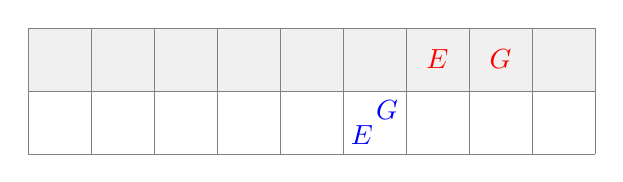
\begin{tikzpicture}[scale=0.8]

\filldraw[ultra thin, lightgray] (0,1) rectangle (9,2);
\draw [help lines] (0,0) grid (9, 2);

\node(e1) at (5.3, 0.3){\textcolor{blue}{$E$}};
\node(g1) at (5.7, 0.7){\textcolor{blue}{$G$}};
\node(e2) at (6.5, 1.5){\textcolor{red}{$E$}};
\node(g2) at (7.5, 1.5){\textcolor{red}{$G$}};

\end{tikzpicture}
\caption{}
\end{subfigure}


\begin{subfigure}[b]{8.1cm}
\centering
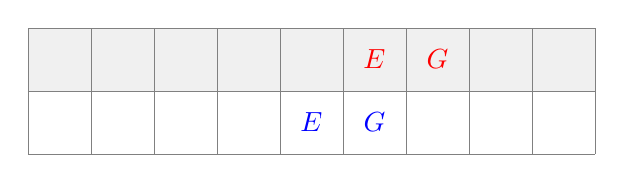
\begin{tikzpicture}[scale=0.8]

\filldraw[ultra thin, lightgray] (0,1) rectangle (9,2);
\draw [help lines] (0,0) grid (9, 2);
\node(e1) at (4.5, 0.5){\textcolor{blue}{$E$}};
\node(g1) at (5.5, 0.5){\textcolor{blue}{$G$}};
\node(e2) at (5.5, 1.5){\textcolor{red}{$E$}};
\node(g2) at (6.5, 1.5){\textcolor{red}{$G$}};

\end{tikzpicture}
\caption{}
\end{subfigure}


\begin{subfigure}[b]{8.1cm}
\centering
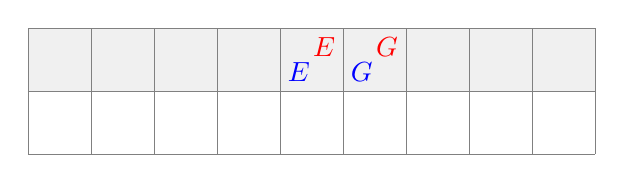
\begin{tikzpicture}[scale=0.8]

\filldraw[ultra thin, lightgray] (0,1) rectangle (9,2);
\draw [help lines] (0,0) grid (9, 2);
\node(e1) at (4.3, 1.3){\textcolor{blue}{$E$}};
\node(g1) at (5.3, 1.3){\textcolor{blue}{$G$}};
\node(e2) at (4.7, 1.7){\textcolor{red}{$E$}};
\node(g2) at (5.7, 1.7){\textcolor{red}{$G$}};

\end{tikzpicture}
\caption{}
\end{subfigure}


\begin{subfigure}[b]{8.1cm}
\centering
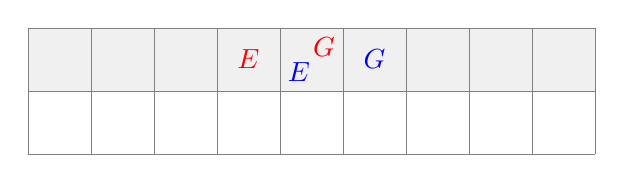
\begin{tikzpicture}[scale=0.8]

\filldraw[ultra thin, lightgray] (0,1) rectangle (9,2);
\draw [help lines] (0,0) grid (9, 2);
\node(e1) at (4.3, 1.3){\textcolor{blue}{$E$}};
\node(g1) at (5.5, 1.5){\textcolor{blue}{$G$}};
\node(e2) at (3.5, 1.5){\textcolor{red}{$E$}};
\node(g2) at (4.7, 1.7){\textcolor{red}{$G$}};

\end{tikzpicture}
\caption{}
\end{subfigure}


\begin{subfigure}[b]{8.1cm}
\centering
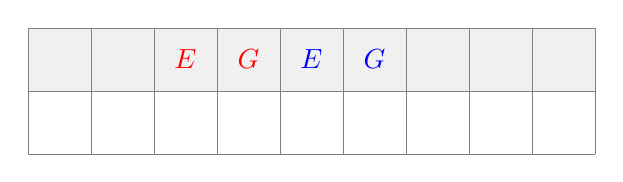
\begin{tikzpicture}[scale=0.8]

\filldraw[ultra thin, lightgray] (0,1) rectangle (9,2);
\draw [help lines] (0,0) grid (9, 2);
\node(e1) at (4.5, 1.5){\textcolor{blue}{$E$}};
\node(g1) at (5.5, 1.5){\textcolor{blue}{$G$}};
\node(e2) at (2.5, 1.5){\textcolor{red}{$E$}};
\node(g2) at (3.5, 1.5){\textcolor{red}{$G$}};

\end{tikzpicture}
\caption{}
\end{subfigure}


\begin{subfigure}[b]{8.1cm}
\centering
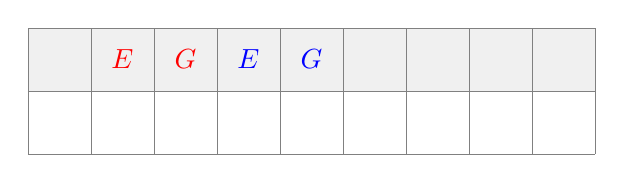
\begin{tikzpicture}[scale=0.8]

\filldraw[ultra thin, lightgray] (0,1) rectangle (9,2);
\draw [help lines] (0,0) grid (9, 2);
\node(e1) at (3.5, 1.5){\textcolor{blue}{$E$}};
\node(g1) at (4.5, 1.5){\textcolor{blue}{$G$}};
\node(e2) at (1.5, 1.5){\textcolor{red}{$E$}};
\node(g2) at (2.5, 1.5){\textcolor{red}{$G$}};

\end{tikzpicture}
\caption{}
\end{subfigure}
\end{multicols}

\caption{}
\end{figure}

At this point, we have an algorithm which will locate the treasure under the three original assumptions. We will hold off on analyzing the runtime of the algorithm until we have described the entire algorithm. In the following section, we describe how to modify the algorithm so it works even when we lift the assumptions.

\section{Separation Phase}

In this section, we will describe the \textit{Separation Phase} of the algorithm. This will be the first phase which is performed. At the start of this phase, all agents are located at the origin.

%Now, we describe how to lift our assumptions. First, we describe an addition to the algorithm which allow us to lift assumptions 1 and 3. We will do this by having the agents perform a routine before they begin executing the algorithm described in the previous section. This routine will be broken into two phases. In phase I, agents will essentially line up to enter phase II. In phase II, the agents will determine their roles for the rest of the algorithm.

First, we introduce a new definition. Define the point $(1, 1)$ to be the \textit{center}. Instead of centering our search around the origin, we will center it around the center (soon we will see why this is necessary). We will redefine level $d$ to be the set of points exactly $d$ steps from the center. Since the center is two steps from the origin, this means that we will need to search all the way through level $D + 2$ in order to ensure that the agents have located the treasure.

To begin, in the first time step, we have all agents move one step to the left, to the position $(-1, 0)$. Now, each time step, we have the agents move to the left with probability 1/2 (and otherwise stay in the same cell). Once an agent finds itself alone in a cell, it takes a step to the right every time step until it reaches the origin. For reasons we will see later, we only want an agent returning to the origin at most once every other time step. Thus, during this phase, the agents will move only on even time steps. Once an agent has returned to the origin, it has completed the \textit{Separation Phase}, and moves directly into the \textsc{Allocation Phase}.

\section{Allocation Phase}

In this section we describe the \textsc{Allocation Phase}. There are two parts to this phase, \textit{Part A} and \textit{Part B}. Each agent completes either \textit{Part A} or \textit{Part B}. The agent decides which part to execute based on whether it is alone at the origin when it enters the \textit{Allocation Phase}. If it is alone, it begins executing \textit{Part B}. Otherwise, it begins executing \textit{Part A}.

\begin{figure}
\footnotesize
\centering
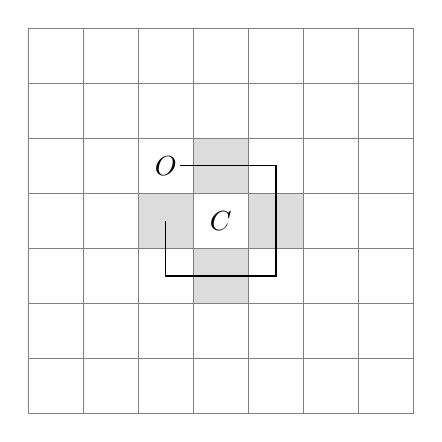
\begin{tikzpicture}[scale=0.7]

\fill[mediumgray] (3, 4) rectangle (4, 5);
\fill[mediumgray] (4, 3) rectangle (5, 4);
\fill[mediumgray] (3, 2) rectangle (4, 3);
\fill[mediumgray] (2, 3) rectangle (3, 4);
\draw [help lines] (0,0) grid (7, 7);
\node(o) at (2.5, 4.5) {$O$};
\node(c) at (3.5, 3.5) {$C$};
\draw  (2.75, 4.5)
    -- (3.5, 4.5)
    -- (4.5, 4.5)
    -- (4.5, 3.5)
    -- (4.5, 2.5)
    -- (3.5, 2.5)
    -- (2.5, 2.5)
    -- (2.5, 3.5);

\end{tikzpicture}
\caption{}
\end{figure}

\subsection{Part B} The first few agents to enter the \textit{Allocation Phase} will actually execute \textit{Part A}. However, it is not clear why \textit{Part A} is necessarily until we describe \textit{Part B}, so we describe \textit{Part B} first.

Say that an agent enters the \textit{Allocation Phase} and finds that it is not alone at the origin. Then it begins to execute \textit{Part B}. To do so, it follows the path outlined in Figure 2.1. Say that an agent takes the first step past the origin and finds itself alone. This will indicate to the agent that it is going to be a north agent. We want the next four agents that pass to know that they are not meant to be north agents. So, that agent will wait until it has been passed by four other agents. For any agent who passes that square and finds itself not alone, it will know it is not a north agent and continue moving along the path.

Once the designated north agent has been passed by four agents, it knows that the rest of its team has passed, and takes a step north. At this point, that agent has completed the \textit{Allocation Phase} and entered the \textit{Search Phase}, so it behaves just like an agent in Section 2 having just left the origin.

The east and south agents are designated the same way. If an agent reaches the cell directly to the right of the center and finds it unoccupied, it knows it will become an east agent and waits for three other agents to pass before moving outwards and entering the \textit{Search Phase}. If an agent reaches the cell directly south of the center and finds it unoccupied, it knows it will become a south agent and waits for two other agents to pass before moving south and entering the \textit{Search Phase}.

The west agent is slightly different. If an agent reaches the cell to the left of the center and finds it unoccupied, it knows it will become the west agent. Then, it waits for an agent to pass by it. Instead of entering the \textit{Search Phase} at that time step, it waits one extra time step in the same place, and then moves left and enters the \textit{Search Phase}.

As soon as an agent reaches the step to the left of the center and finds it occupied, that agent knows it is an explorer, and it takes a step to the left in the next time step, also entering the \textit{Search Phase}. By waiting a single extra time step, the west guide ensures that it does not walk out on top of the explorer, in which case neither could sense if they were in the presence of other agents. Note that because agents only enter the \textit{Allocation Phase} every other time step, it is impossible for another agent to encounter a west agent while it is waiting that extra time step before entering the \textit{Search Phase}.

Figure 2.2 shows a sample execution of \textit{Part B} on five agents. Since the \textit{Separation Phase} involved randomness, we display an execution where we assume that the agents executed the \textit{Separation Phase} in such a way that they end up entering the \textit{Allocation Phase} exactly once every other time step. Note that the figure displays only even time steps.


\begin{figure}
\footnotesize

\begin{multicols}{3}
\begin{subfigure}[b]{.3\textwidth}
\centering
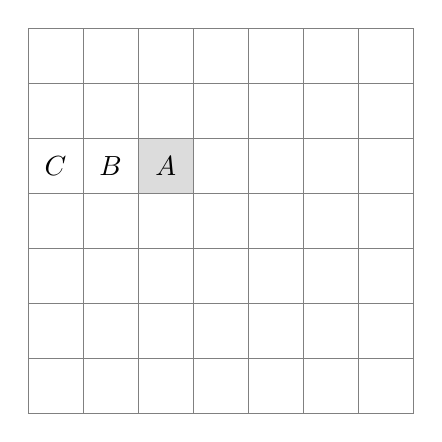
\begin{tikzpicture}[scale=0.7]

\fill[mediumgray] (2, 4) rectangle (3, 5);
\draw [help lines] (0,0) grid (7, 7);
\node(1) at (2.5, 4.5){$A$};
\node(2) at (1.5, 4.5){$B$};
\node(3) at (0.5, 4.5){$C$};

\end{tikzpicture}
\caption{$t = 0$}
\end{subfigure}

\begin{subfigure}[b]{.3\textwidth}
\centering
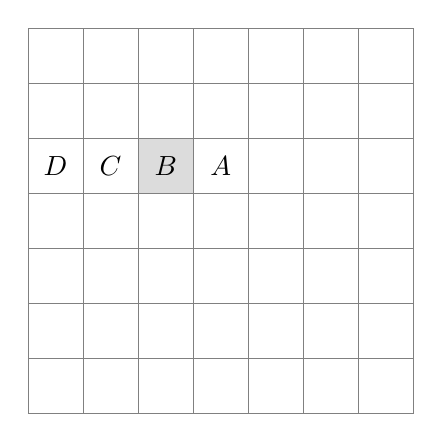
\begin{tikzpicture}[scale=0.7]

\fill[mediumgray] (2, 4) rectangle (3, 5);
\draw [help lines] (0,0) grid (7, 7);
\node(a) at (3.5, 4.5){$A$};
\node(b) at (2.5, 4.5){$B$};
\node(c) at (1.5, 4.5){$C$};
\node(d) at (0.5, 4.5){$D$};

\end{tikzpicture}
\caption{$t = 2$}
\end{subfigure}


\begin{subfigure}[b]{.3\textwidth}
\centering
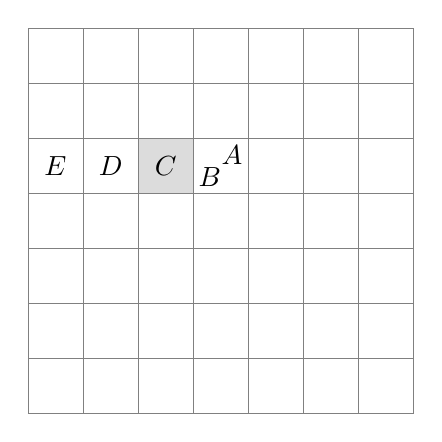
\begin{tikzpicture}[scale=0.7]

\fill[mediumgray] (2, 4) rectangle (3, 5);
\draw [help lines] (0,0) grid (7, 7);
\node(a) at (3.7, 4.7){$A$};
\node(b) at (3.3, 4.3){$B$};
\node(c) at (2.5, 4.5){$C$};
\node(d) at (1.5, 4.5){$D$};
\node(e) at (0.5, 4.5){$E$};

\end{tikzpicture}
\caption{$t = 4$}
\end{subfigure}


\begin{subfigure}[b]{.3\textwidth}
\centering
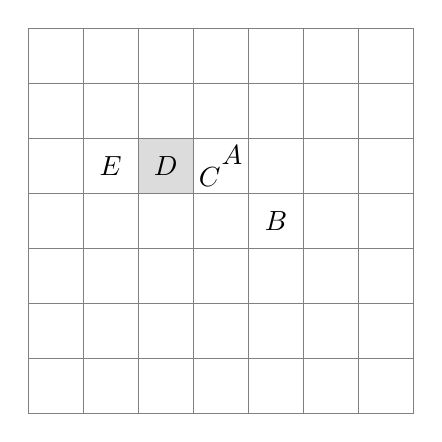
\begin{tikzpicture}[scale=0.7]

\fill[mediumgray] (2, 4) rectangle (3, 5);
\draw [help lines] (0,0) grid (7, 7);
\node(a) at (3.7, 4.7){$A$};
\node(b) at (4.5, 3.5){$B$};
\node(c) at (3.3, 4.3){$C$};
\node(d) at (2.5, 4.5){$D$};
\node(e) at (1.5, 4.5){$E$};

\end{tikzpicture}
\caption{$t = 6$}
\end{subfigure}


\begin{subfigure}[b]{.3\textwidth}
\centering
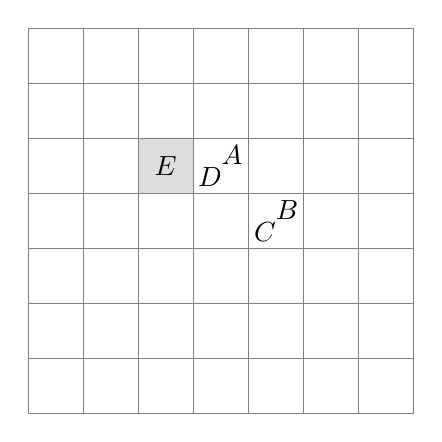
\begin{tikzpicture}[scale=0.7]

\fill[mediumgray] (2, 4) rectangle (3, 5);
\draw [help lines] (0,0) grid (7, 7);
\node(a) at (3.7, 4.7){$A$};
\node(b) at (4.7, 3.7){$B$};
\node(c) at (4.3, 3.3){$C$};
\node(d) at (3.3, 4.3){$D$};
\node(e) at (2.5, 4.5){$E$};

\end{tikzpicture}
\caption{$t = 8$}
\end{subfigure}


\begin{subfigure}[b]{.3\textwidth}
\centering
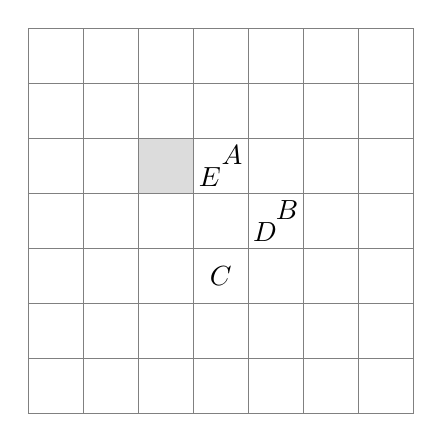
\begin{tikzpicture}[scale=0.7]

\fill[mediumgray] (2, 4) rectangle (3, 5);
\draw [help lines] (0,0) grid (7, 7);
\node(a) at (3.7, 4.7){$A$};
\node(b) at (4.7, 3.7){$B$};
\node(c) at (3.5, 2.5){$C$};
\node(d) at (4.3, 3.3){$D$};
\node(e) at (3.3, 4.3){$E$};

\end{tikzpicture}
\caption{$t = 10$}
\end{subfigure}


\begin{subfigure}[b]{.3\textwidth}
\centering
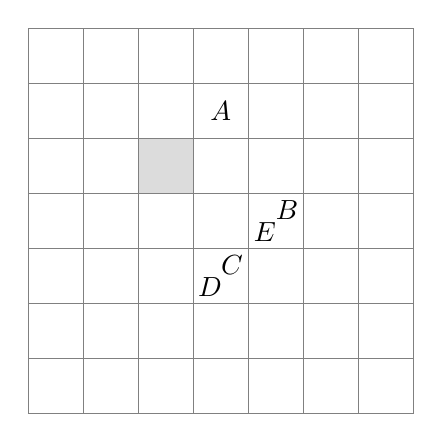
\begin{tikzpicture}[scale=0.7]

\fill[mediumgray] (2, 4) rectangle (3, 5);
\draw [help lines] (0,0) grid (7, 7);
\node(a) at (3.5, 5.5){$A$};
\node(b) at (4.7, 3.7){$B$};
\node(c) at (3.7, 2.7){$C$};
\node(d) at (3.3, 2.3){$D$};
\node(e) at (4.3, 3.3){$E$};

\end{tikzpicture}
\caption{$t = 12$}
\end{subfigure}

\begin{subfigure}[b]{.3\textwidth}
\centering
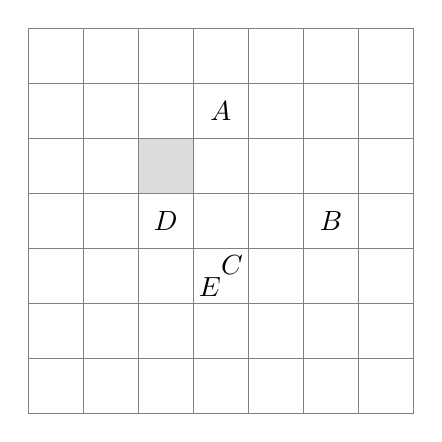
\begin{tikzpicture}[scale=0.7]

\fill[mediumgray] (2, 4) rectangle (3, 5);
\draw [help lines] (0,0) grid (7, 7);
\node(a) at (3.5, 5.5){$A$};
\node(b) at (5.5, 3.5){$B$};
\node(c) at (3.7, 2.7){$C$};
\node(d) at (2.5, 3.5){$D$};
\node(e) at (3.3, 2.3){$E$};

\end{tikzpicture}
\caption{$t = 14$}
\end{subfigure}


\begin{subfigure}[b]{.3\textwidth}
\centering
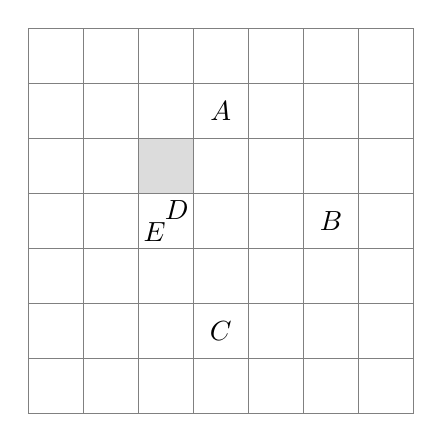
\begin{tikzpicture}[scale=0.7]

\fill[mediumgray] (2, 4) rectangle (3, 5);
\draw [help lines] (0,0) grid (7, 7);
\node(a) at (3.5, 5.5){$A$};
\node(b) at (5.5, 3.5){$B$};
\node(c) at (3.5, 1.5){$C$};
\node(d) at (2.7, 3.7){$D$};
\node(e) at (2.3, 3.3){$E$};

\end{tikzpicture}
\caption{$t = 16$}
\end{subfigure}


\begin{subfigure}[b]{.3\textwidth}
\centering
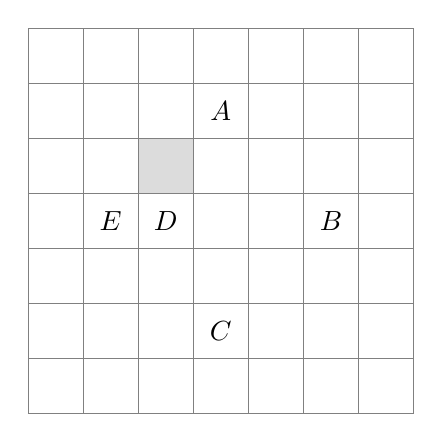
\begin{tikzpicture}[scale=0.7]

\fill[mediumgray] (2, 4) rectangle (3, 5);
\draw [help lines] (0,0) grid (7, 7);
\node(a) at (3.5, 5.5){$A$};
\node(b) at (5.5, 3.5){$B$};
\node(c) at (3.5, 1.5){$C$};
\node(d) at (2.5, 3.5){$D$};
\node(e) at (1.5, 3.5){$E$};

\end{tikzpicture}
\caption{$t = 18$}
\end{subfigure}


\begin{subfigure}[b]{.3\textwidth}
\centering
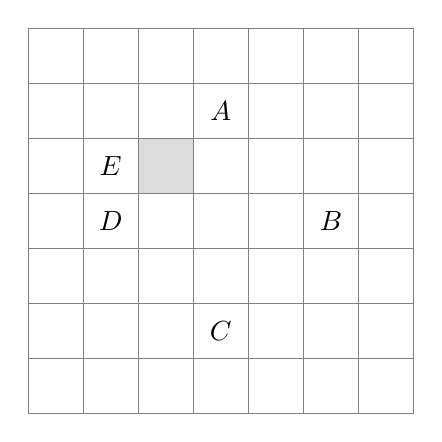
\begin{tikzpicture}[scale=0.7]

\fill[mediumgray] (2, 4) rectangle (3, 5);
\draw [help lines] (0,0) grid (7, 7);
\node(a) at (3.5, 5.5){$A$};
\node(b) at (5.5, 3.5){$B$};
\node(c) at (3.5, 1.5){$C$};
\node(d) at (1.5, 3.5){$D$};
\node(e) at (1.5, 4.5){$E$};

\end{tikzpicture}
\caption{$t = 20$}
\end{subfigure}


\begin{subfigure}[b]{.3\textwidth}
\centering
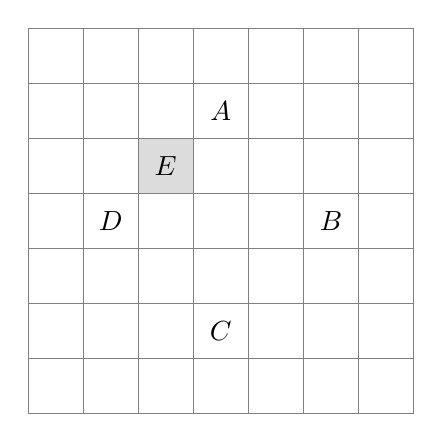
\begin{tikzpicture}[scale=0.7]

\fill[mediumgray] (2, 4) rectangle (3, 5);
\draw [help lines] (0,0) grid (7, 7);
\node(a) at (3.5, 5.5){$A$};
\node(b) at (5.5, 3.5){$B$};
\node(c) at (3.5, 1.5){$C$};
\node(d) at (1.5, 3.5){$D$};
\node(e) at (2.5, 4.5){$E$};

\end{tikzpicture}
\caption{$t = 22$}
\end{subfigure}

\end{multicols}

\caption{TEST}
\end{figure}

At this point, we should note that we have shown that Assumptions 1 and 3 are valid *** MAKE EXTRA ASSUMPTION?? **. Each agent that enters the search team knows its role, and a team member of each role enters the \textit{Search Phase} at least twelve units after the previous.

We are left with a final issue of dealing with the fact that currently, we need the agents to know whether they are the first team to enter the \textit{Search Phase}. In Figure 2.2, we see that the guides all stop exactly two steps from the center, and the explorer begins searching level 2. However, they must know that they are the first team in order to do that. Recall that agents from every subsequent team walk away from the origin until they find an empty even cell \textit{after} having passed by another agent. Of course, the first team cannot do this because they will never encounter another agent and therefore walk on forever.

\subsection{Part B} This problem is solved by the introduction of \textit{Part A}. Recall that an agent that has just entered the \textit{Allocation Phase} will begin executing \textit{Part A} if it finds itself alone at the origin. Since no agents from the \textit{Separation Phase} can remain at the origin, the first agent to enter the \textit{Allocation Phase} will immediately enter \textit{Part A}. As we will see, an agent entering \textit{Part A} immediately steps away from the origin. As a result, the next agent to enter the \textit{Allocation Phase} will also be alone at the origin. This process will repeat until some \textit{Part A} agent returns to the origin. At this point, all agents entering the \textit{Allocation Phase} will begin executing \textit{Part B}.

\textit{Part A} is very similar to \textit{Part B}. The agents will walk along a predetermined course. If they find themselves alone in certain cells, they will stop and wait there until some condition indicates to them that they can move forward. Figure xx shows that path that agents execute in \textit{Part A}. As in Figure xx, the gray cells show the ones in which agents stop in if they find themselves there alone.


\begin{figure}
\footnotesize
\centering
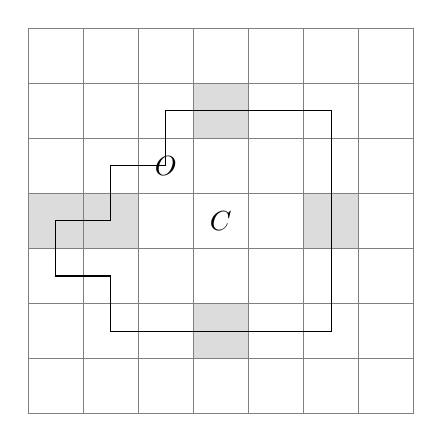
\begin{tikzpicture}[scale=0.7]

\fill[mediumgray] (3, 5) rectangle (4, 6);
\fill[mediumgray] (5, 3) rectangle (6, 4);
\fill[mediumgray] (3, 1) rectangle (4, 2);
\fill[mediumgray] (0, 3) rectangle (2, 4);
\draw [help lines] (0,0) grid (7, 7);
\node(o) at (2.5, 4.5) {$O$};
\node(c) at (3.5, 3.5) {$C$};
\draw  (2.5, 4.5)
    -- (2.5, 5.5)
    -- (3.5, 5.5)
    -- (4.5, 5.5)
    -- (5.5, 5.5)
    -- (5.5, 4.5)
    -- (5.5, 3.5)
    -- (5.5, 2.5)
    -- (5.5, 1.5)
    -- (4.5, 1.5)
    -- (3.5, 1.5)
    -- (2.5, 1.5)
    -- (1.5, 1.5)
    -- (1.5, 2.5)
    -- (0.5, 2.5)
    -- (0.5, 3.5)
    -- (1.5, 3.5)
    -- (1.5, 4.5)
    -- (2.5, 4.5);

\end{tikzpicture}
\caption{}
\end{figure}

If an agent passes by all five gray cells and finds them occupied, then it continues along the path and returns to the origin. After this point, there will always be at least one agent at the origin, so all subsequent agents entering the \textit{Allocation Phase} will execute \textit{Part B}. We will also note that in the worst case (where agents are entering the \textit{Allocation Phase} every other time step), there can be at most $13$ agents which begin executing \textit{part A} before one of them returns to the origin. This means at most $8$ agents will return to the origin. Note that any agent who executes \textit{Part A} and returns to the origin will never leave the origin again.

Now, when an agent enters \textit{Part B}, it can just assume that it is not on the first team. This is because the \textit{Part A} agents will still be positioned in their gray spots, and so even the first \textit{Part B} team will pass by them and know that they can search the next unoccupied level.

The problem is once the agents start completing their levels and moving outwards. If there are still agents in \textit{Separation} and \textit{Allocation Phases} at that time, we do not want them to re-search early levels after seeing the \textit{Part A} agents positioned at level 2.

The real purpose of the \textit{Part A} team is to ensure that the first \textit{Part B} team does not wander away. So, once that team has passed, we can have the \textit{A} agents enter the \textit{Search Phase}. It remains to show how the \textit{Part A} agents know the difference between the first search team passing by them, and just another \textit{Part A} agent making its way around. To resolve this, we note that agents only enter \textit{Part A} every other step.

When the first search team begins to move outwards, it will encounter agents at level 2. Only \textit{Part A} agents will ever be stopped there, so it will know the agents are \textit{Part A} agents. The new search team will then wait in the cells with the \textit{Part A} agents for an extra time step before proceeding. This will signal to the \textit{Part A} agents that they have been passed by a search team. After that search team steps away, the \textit{Part A} agents can enter the \textit{Search Phase}, with their roles determined by their positions.

Note that all level 1, 2, and 3 cells are searched by \textit{Allocation Phase} agents except for the level 3 cells on the axes. Since these will be search by guides in the \textit{Search Phase}, there is no need to ever have a team explore these levels. We have to be careful because no agent ever actually explores the center. To fix this, we just have all the agents move to the center and back to the origin before beginning the \textit{Separation Phase}.

\section{Analysis}

\begin{thm}
\textsc{Rectangle-Search} locates the treasure in $O(D + D^2/k + \log{k})$ with high probability.
\end{thm}

\begin{proof}
First, we need to analyze the rate at which agents complete the \textit{Separation Phase}. To do so, we use the following lemma.

\begin{lem}
After $O(t + \log{k})$ time steps, at least $t$ agents have completed the \textit{Separation Phase} with high probability.
\end{lem}

\begin{proof}
Still need to work this out exactly. The general idea is that is takes $O(\log{k})$ steps for one of the agents to become alone, and after that happens we expect roughly one agent to become alone every time step. Very roughly.
\end{proof}

%Next, we assess the time until one of the Phase X agents return to the origin (which marks the point at which Phase I agents start moving into Phase II). As we've stated before, at most 13 agents can enter Phase X before one of them winds up back at the origin. Once the last agent enters phase X, it will take at most a constant number of steps before some phase X agent reaches the origin. Thus, by Lemma xx, we expect this to happen in $O(\log{k})$.

Define team $0$ to be the team which is formed in \textit{Part A}, and define team $i$ to be the $i^{th}$ team formed in phase \textit{B}. Next, we will define team $j$ to be the last team to enter the \textit{Search Phase}. Since the agents move in synchrony, the runtime of the algorithm is equal to the number of steps taken by team $j$.

\begin{lem} We must have that $j = O(D)$.
\end{lem}

\begin{proof}
Even if each team only explored a single level, the $D/2^{th}$ team would end up exploring level $D$. After $O(D)$ time steps, that team would complete exploration of level $D$ and the algorithm would terminate. Since at most one team can start per time step, this leads to $j = O(D)$. 
\end{proof}

Let $m$ be the maximum number of possible teams that can be formed from the $k$ agents. Recall that at least $1$ and at most $8$ agents will complete \textit{Part A} and then return to the origin to never leave again. So, we have that $\lfloor (k - 8)/5 \rfloor \leq m \leq \lfloor (k - 1)/5 \rfloor$, and $m = \Theta(k)$.

We analyze two cases. In the first case, $j = m$. This corresponds to the case where $D$ is large compared to $k$, so all possible teams are deployed and join the search before the treasure is found. In the second case, $j < m$. This corresponds to the case where $D$ is small compared to $k$, so the treasure is located before all the teams are deployed.

\begin{lem} If $j = m$, then the algorithm terminates after $O(D + D^2/k)$ steps with high probability.
\end{lem}

\begin{proof}
This means that $D$ was large enough such that all the agents completed the \textit{Separation} and \textit{Search Phases} and participated in the \textit{Search Phase}. By Lemma xx, it takes $O(k + \log{k}) = O(k)$ time steps with high probability before team $m$ completes the \textit{Separation Phase}. Note at after the final agent on a team completes \textit{Separation Phase}, it only takes a constant number of steps before that team moves on to the \textit{Search Phase}.

When a team enters the \textit{Search Phase}, it moves out to find the first unexplored level. Say that this is level $f$. Once there, the team explores that level. Recall that it takes $O(d)$ steps to explore level $d$. So, in $O(f)$ steps, the team explores level $f$. Next, they move out and explore the next unexplored level, which will be level $f + 2m$. After exploring that level, they will move out and explore level $f + 4m$. This process can repeat at most $D/2m$ times. So, the total amount of work is given by the following sum.

\[f + \sum_{z = 0}^{D/(2m)} O(f + z \cdot (2m)) + m\]
\[= f + O \left (\sum_{z = 0}^{D/k} f + zk \right )\]
\[= f + O \left (\sum_{z = 0}^{D/k} f + k\sum_{z = 0}^{D/k} z \right ) \]
\[= f + O((D/k)\cdot f + D^2/k)\]

To simplify this further, we claim that $f = O(D)$. To see why, we note that if $f > D$, then it means that by the time that team $j$ starts its search, some other team is already searching level $D$. That team will complete its search within $O(D)$ steps of the time when team $j$ begins its search, so team $j$ cannot possibly start a search further than $O(D)$ steps from the origin. With this in mind, the above sum simplifies to

\[= O(D + D^2/k + D^2/k) = O(D + D^2/k)\]

With this, the total time before the algorithm terminates is
\[O(D + D^2/k + k).\]
By Lemma xx, $k = O(D)$, so we have that the overall runtime is given by $O(D + D^2/k)$ with high probability.
\end{proof}

\begin{lem} If $j < m$, then the algorithm terminates after $O(D + \log{k})$ steps with high probability.
\end{lem}

\begin{proof}
This means that not all teams completed the \textit{Separation} and \textit{Allocation Phases} by the time that some team located the treasure.

We know that team $j + 1$ never completes the \textit{Allocation Phase}, because the algorithm terminates before this. By Lemma xx, this team would have completed the \textit{Separation Phase} in $O(j + \log{k})$ time steps with high probability. Since the \textit{Allocation Phase} only involves a constant number of steps after the final agent of the team enters that phase, this means that team $j + 1$ also would have completed the \textit{Allocation Phase} in $O(j + \log{k})$. Thus, the algorithm completes in $O(j + \log{k})$ with high proability. Then by Lemma xx, the algorithm completes in $O(D + \log{k})$ with high probability.
\end{proof}

Combining Lemmas xx and xx, we have that the algorithm terminates in $O(D + D^2/k + \log{k})$ with high probability.

%Let us consider the total time some team spends in \textit{Phase III}. Once a team enters \textit{Phase III}, it has to walk until it discovers the first level that it is going to search. Say that the first level searched by team $i$ is level $f_i$.

%Next the team searches that level. Recall that it takes $O(d)$ steps to search level $d$. Once the team completes that level, it walks out to the next unexplored level. At most, there are $k/5$ teams out searching at once. Since teams only search every other level, this means that the furthest a team will ever have to walk to reach the next level it wants to search is $2k/5$.

%Recall that once a team leaves the origin, it searches the nearest unexplored level, and then immediately moves outwards to search the next nearest unexplored level. Recall that there are $k/5$ teams. Instead of our current algorithm, imagine if we just had the teams split up the levels so that each team explored every $2k/5^{th}$ level. So we would have team 1 explore levels $2$, $2k/5 + 2$ , $4k/5 + 2$, $\hdots$, team 2 explore levels $4$, $2k/5 + 4$, $4k/5 + 4$, etc., so that team $k/5$ would explore levels $2k/5$, $4k/5$, $6k/5$.

%We claim that this algorithm would be strictly slower than our algorithm at covering all levels through level $D + 2$. This is because in our algorithm, we always search level $d$ before anyone searches level $d + 1$. In the suggested algorithm, team $1$ could be searching some level way past level $D + 2$ while there are still levels before $D + 2$ waiting to be searched.

%However, this algorithm is still useful to consider, because we claim that it operates asymptotically equally to the desired time, yet it is simpler to analyze. So, we will show that this algorithm works in the desired time, and then claim that our algorithm does as well.


%Consider some team $i$. It first explores distance $i$. Next, it explores distance $i + k/5$, because it walks past all other search teams before beginning its next exploration. It continues this process until the treasure is found, which will happen by the time some team explores distance $D$. The total number of distances that any one team can explore until this happens is $D/(k/5)$. Finally, using the fact that an explorer takes $8d$ steps to explore distance $d$, we see that the total number of steps some \textit{explorer} spends exploring is
%\begin{equation*}
%\begin{split}
%\sum_{z = 0}^{D/(k/5)} 8 \left (i +  z \cdot \left (\frac{k}{5} \right )\right)
%&= O \left ( \sum_{z = 0}^{D/k} i + zk \right )\\
%&= O \left ( \sum_{z = 0}^{D/k} i + k\cdot \sum_{z = 0}^{D/k} z \right )\\
%&= O(D + D^2/k)
%\end{split}
%\end{equation*}
%Thus, the total number of steps spent by team $i$ is $O(D + D^2/k + i + \log{k})$ with high probability. We make the final note that $i = O(D + D^2/k)$. To see why, we can see that even if we had an unlimited number of search teams and we were able to start a new search team every step, the total number of search teams started before the treasure was found would be no more than the total number of steps taken to find the treasure. With this in mind, the total number of steps to find the treasure is $O(D + D^2/k + \log{k})$ with high probability.

\end{proof}




\end{document}
